%*******************************************************************************
%***************************** Finite difference Chapter ***********************
%*******************************************************************************

\chapter{Finite Difference Method}

%------------------Introduction-------------------------------
\section{Introduction}
The finite difference approximation for derivativatives is one of the simplest oldest method to solve differential equations numerically. It was used since 1768 by \textit{L. Euler} to solve one dimensional problem and extended by \textit{C. Runge} to two dimension in 1910 ca. Since the advent of computers in 1950 ca. FDM  popularity skyrocketed and during the last five decades theoretical results have been obtained regarging stability, convergence and other of its properties.



    The general idea behind FDM is that the differential operator is approximated by replacing the derivatived using difference quotients, which are linear combination of function values at the grid points). In order to do so the space and time domain are \textit{partitioned} in a grid like fashion and approximated solutions are computed only for those discrete grid points. The numerical solution is known only at a finite number of points in the physical domain.
    Figure \ref{fig:schematic_repr_fdm} is a schematic representation of how FDM are used to obtain a numerical solution.
    \begin{figure}
    \centering
    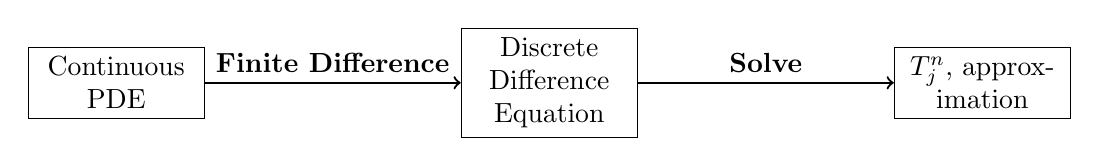
\begin{tikzpicture}

    \node[draw, text centered,text width=2cm] (1) at (0,0) {Continuous PDE};
    \node[draw, text centered,text width=2cm] (2) at (5.5,0) {Discrete Difference Equation};
    \node[draw, text centered,text width=2cm] (3) at (11,0) {$T_j^n$, approximation};

\draw[thick,->] (1) -- (2) node[midway,sloped,above,rotate=0] {\textbf{Finite Difference}};
\draw[thick,->] (2) -- (3) node[midway,sloped,above,rotate=0] {\textbf{Solve}};
\end{tikzpicture}
    \caption{Relationship between continuous and discrete problems.}
    \label{fig:schematic_repr_fdm}
\end{figure}
    
    The error, between the numerical solution and the exact solution is determined by the difference formula utilized and is commonly refeered as \textit{truncation}\footnote{The term truncation comes from the fact that a finite difference quotient is a truncation of the Taylor expansion.} or \textit{discretization} error.  Increasing the resoution of the grid increases the accuracy of the numerical solution since the error associated with the finite difference formulas depends on the distance between grid points.
    
        
    Depending on how the derivatives are approximated, explicit or implicit FDM schemes are
    obtained. When forward difference formulas are considered, the
    resulting difference equation is generally expressed in terms of
    an explicit recurrence formula, while backward difference formulas
    generally lead to implicit recurrence formulas involving unknown
    values, and therefore require the solution of a linear system to
    obtain the new state of the system at each grid point.
    
    
     %------------------Finite difference Formulas-------------------------------
    \section{Finite difference formulas}


    
    Difference formulas can be derived from Tailor's expansion of $T^n_{j+1}$ in terms of $T^n_{j}$ and its derivatives as:
    
    \begin{equation}
    T^n_{j+1} = T^n_{j} +
    \frac{\partial T(t,x)}{\partial x}\bigg\rvert^n_j \Delta x +
    \frac{1}{2!}  \frac{\partial^2 T(t,x)}{\partial x^2}\bigg\rvert^n_j \Delta x^2 + \ldots + 
     \frac{1}{k!}  \frac{\partial^k T(t,x)}{\partial x^k}\bigg\rvert^n_j \Delta x^k + \ldots
     \label{eq:taylorexp1}
    \end{equation}
    
    If series is truncated after the second term ($k=1$) and solving for $\frac{\partial T(t,x)}{\partial x}$ the following is obtained:
    
    \begin{equation}
    \frac{\partial T(t,x)}{\partial x}  = \frac{T^n_{j+1} - T^n_{j}}{\Delta x}
    \label{eq:fdmforward}
    \end{equation}
    
    Equation \ref{eq:fdmforward} is called fist \textbf{forward} finite difference approximation. Other approximations are possible and are easilby obtainable by expanding different points of the grids and using more points from the expansion.
    
    \textbf{Backward} finite difference quotient can be obtained from the Taylor's expansions of    
        \begin{equation}
    T^n_{j-1} = T^n_{j} - 
    \frac{\partial T(t,x)}{\partial x}\bigg\rvert^n_j \Delta x +
    \frac{1}{2!}  \frac{\partial^2 T(t,x)}{\partial x^2}\bigg\rvert^n_j \Delta x^2 + \ldots + 
     \frac{1}{k!}  \frac{\partial^k T(t,x)}{\partial x^k}\bigg\rvert^n_j \Delta x^k + \ldots
     \label{eq:taylorexp2}
    \end{equation}
    
    which can be rearranged in the following manner
        \begin{equation}
    \frac{\partial T(t,x)}{\partial x}  = \frac{T^n_{j} - T^n_{j-1}}{\Delta x}
    \label{eq:fdmfbackward}
    \end{equation}
    
   The same approach can be used to derive approximation for higher order derivatives.
   For example equation \ref{eq:fdmcentral}, known called \textbf{central difference formula}, is an approximation for the second order derivative and can be obtained retaining the firsts four terms in both equations \ref{eq:taylorexp1} and \ref{eq:taylorexp2} and adding the resulting expression:
   
    \begin{equation}
		\frac{\partial^2 T(t,x)}{\partial x^2} = \frac{T^n_{j+1}- 2T^n_{j} + T^n_{j-1}}{\Delta x^2}
		\label{eq:fdmcentral}
    \end{equation}
    
    Figure \ref{fig:geometrical_intepretation} show how finite difference formulas can be interpreted geometrically.
    \begin{figure}
\centering
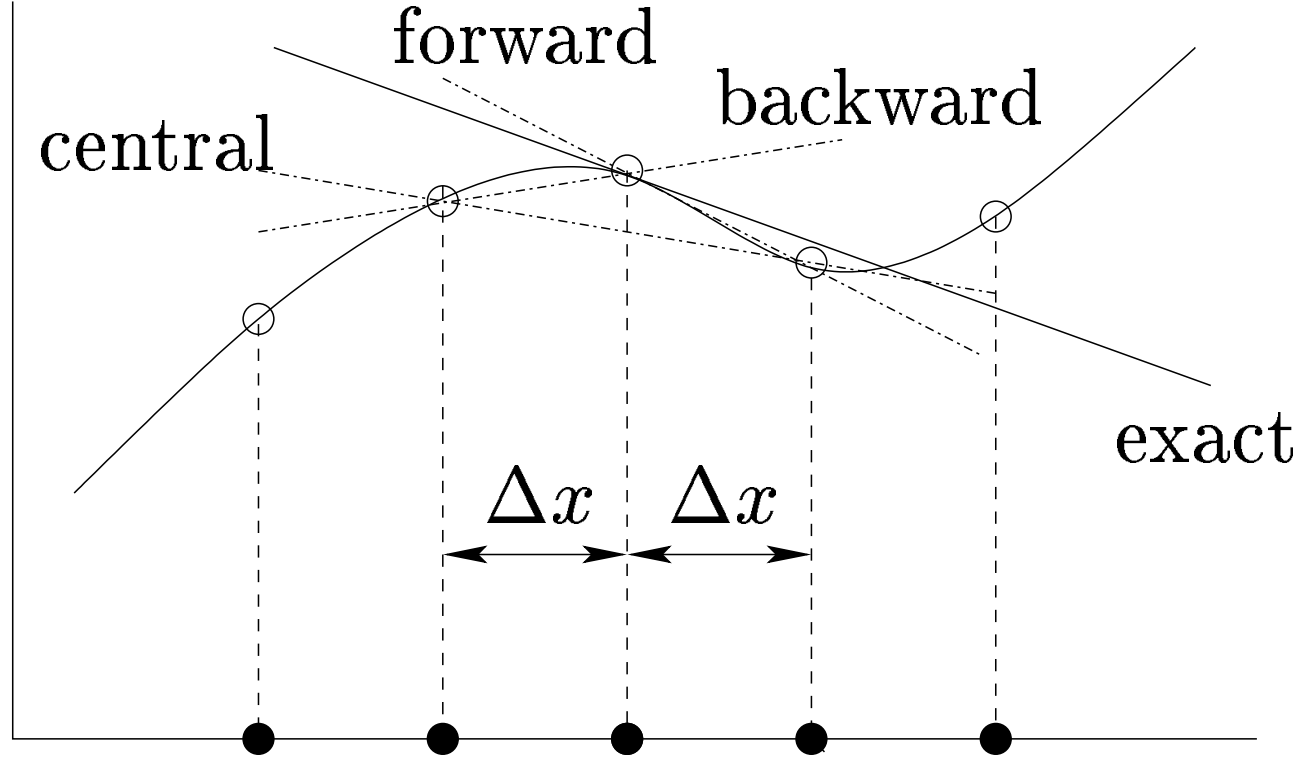
\includegraphics[scale=0.3]{./images/CA_FDM/geometrical_interpretation_fd}
\label{fig:geometrical_intepretation}
\caption{Explicit FDM discretization for the 1D heat conduction problem}\label{torus}
\end{figure} 
    
    %------------------HEAT Equation-------------------------------
    \section{Heat Equation}
        As an example a simple FDM scheme for an initial-boundary condition problem for the heat conduction problem is derived. 
    
\begin{equation}
    \frac{\partial T(t,x)}{\partial t}= k\frac{\partial^2
      T(t,x)}{\partial x^2}
      \label{eq:heatconduction}
\end{equation}
 
    where $0 \leq t \leq L$ and $0 \leq x \leq
    M$. 
 In order to construct a FD approximation for equation \ref{eq:heatconduction} 
 
 \begin{enumerate}
 
 \item Both space and time domain are partitioned into a finite grid as follows:
    
    \begin{equation}
    		x_j = j\Delta x, \: j = 0,1,\ldots,M,\;\Delta x = \frac{1}{M}
    \end{equation}

 \begin{equation}
    		t_n = n\Delta t, \: n = 0,1,\ldots,L,\; \Delta t= \frac{1}{L}
    \end{equation}  
    
 \item  First and second order derivative appearing in \ref{eq:heatconduction} are substituted by forward and central difference formulas respectively leading to (see Figure  \ref{fig:fdmheatequationstencil}):
 
 \begin{equation}
  \frac{T^n_{j+1} - T^n_{j}}{\Delta x} = k \frac{T^n_{j+1}- 2T^n_{j} + T^n_{j-1}}{\Delta x^2}
 \label{eq:discretizedheatequation}
 \end{equation}
 
 \item Equation \ref{eq:heatconduction} is evaluated at grid point $(n\Delta t, j \Delta x)$ 
    
\end{enumerate}    
    
\begin{figure}
\centering
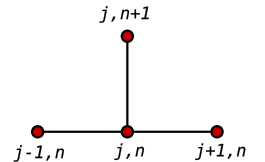
\includegraphics[scale=0.5]{./images/CA_FDM/heatstencil}
\label{fig:fdmheatequationstencil}
\caption{Explicit FDM discretization for the 1D heat conduction problem}\label{torus}
\end{figure}    
    
\begin{figure}
\centering
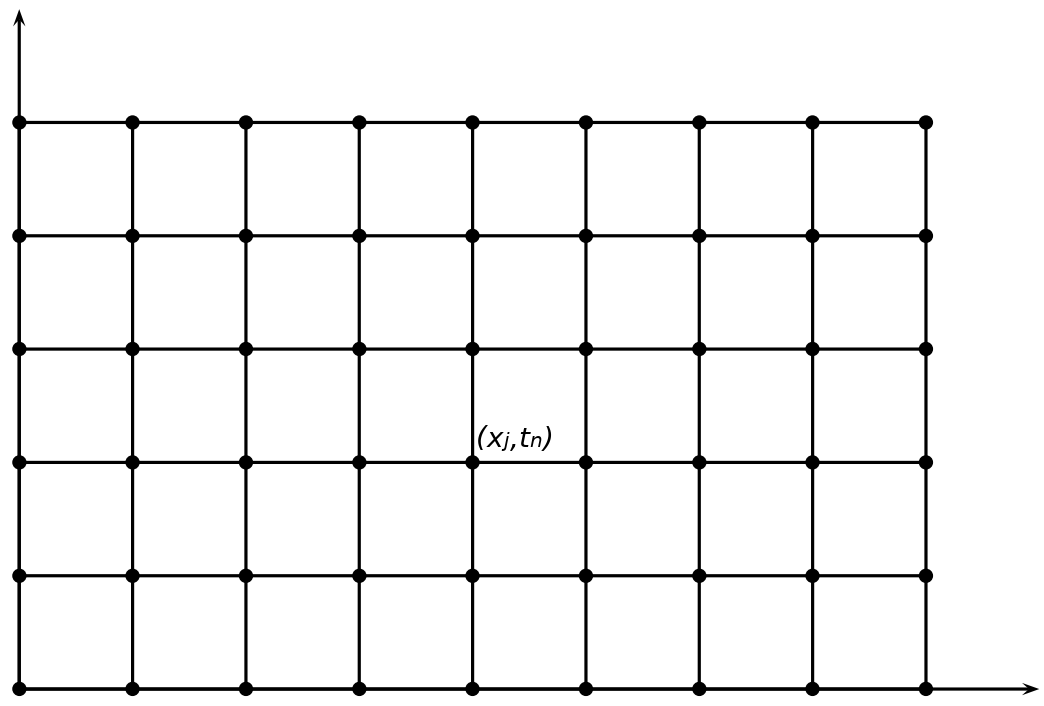
\includegraphics[scale=0.3]{./images/CA_FDM/fdmgrid}
\caption{1D heat equation FDM grid space and time partitioning.}\label{torus}
\end{figure}

Solution to equation \ref{eq:heatconduction} requires the specification of boundary conditions at $t=0$ and $x=0$ and $x=M$.
In this example the temperature in the interior of the domain is assumed to be $0$ i.e. and edges in the $x$ dimension are assumed to be source of constant heat i.e. $T(0, 0<x<M)$,  $T(t,0)=100$, $T(t,M)=100$.
         
    $h = \Delta x = 0.2$ and $\Delta t = 0.01$ with initial
    conditions $T(0, 0 < x < M) = 0$ and boundary conditions $T(0,x=0)
    = 100 \: , u(0,x=L) =100$. Note that, assuming $k=1$, the values
    assigned to the spatial and temporal steps satisfy the von Neumann
    stability analysis. In fact, $\frac{k \Delta t}{\Delta x^2} = 1/4
    \leq 1/2$.
   
        In this example, a one-dimensional cellular space $R$
    can be used (cf. Figure \ref{fig:cellularspaces}a) to model the
    $10$ grid points $i$ $(i = 0, 1, ...,9)$, while the values that
    the generic cell can assume are simply represented by the $Q = [0,
      100] \subset \mathbb{R}$ substate. By using the forward
    difference formula for the first order derivative and the central
    one for the second order, the following explicit recurrence scheme
    is obtained:
    $$ T_i^{t+1} = T_i^t + k \Delta t \frac{T_{i+1}^t - 2T_i^t +
      T_{i-1}^t}{\Delta x^2}
    $$ denoting that the value of the temperature at the grid point
    $i$ at the time step $t+1$ is a function of the (known) values
    assumed by $T$ at the $i-1$, $i$ and $i+1$ grid points at the
    (previous) time step $t$. Thus, the one dimensional radious-one $X
    = \{-1, 0, 1\}$ neighburhood pattern can be adopted (cf. Figure
    \ref{fig:1Dneighborhood}a) and an elementary process used to
    implement the above recurrence scheme. The explicit formulation of
    the FDM one-dimensional heat conduction model can be therefore
    expressed in terms of the XCA formalism as:

    $$ FDM_{heat} = <R,\Gamma,X,Q,P,\sigma,\gamma>$$

    \noindent where:

    \begin{itemize}

    \item $R = \{0,1,...,9\}$ is the one-dimensional cellular space,
      representing the integer coordinates of the cells of the
      computational domain (cf. Figure \ref{fig:cellularspaces}a).

    \item $\Gamma = \{0, 9\} \subset R$ is the region identifying the
      boundary of the computational domain.


    \item $X = \{-1, 0, 1\}$ is the geometrical pattern defining the
      neighborhood relationship (cf. Figure
      \ref{fig:1Dneighborhood}a).

    \item $Q = [0, 100] \subset \mathbb{R}$ is the set of cell's
      states used to express the temperature values at the grid
      points.

    \item $P = \{k = 1, \Delta t = 0.01, \Delta x = 0.2\}$ is the set
      of the FDM model parameters.
      
    \item $\sigma : Q^3 \rightarrow Q$ is the cell's transition
      function, which implements the explicit recurrence FDM scheme.

    \item $\gamma: Q^{|\Gamma|} \rightarrow Q^{|\Gamma|} \times
      \mathbb{R}$ is the global steering function, used to apply the
      boundary conditions at each computational step.

    \end{itemize}

    The initial conditions of the system are preliminarly defined at
    time $t=0$ by assigning the temperature value 0 to each grid
    point, except for the boundaries where the value 100 is set. The
    global evolution of the system can therefore be obtained by
    applying the $\tau$ global transition function (which in turn
    applies $\sigma$ to each grid point) and eventually the steering
    function $\gamma$ at discete time steps.
    
    
    
    
    
        
    %%XCA and finite difference method-----------------------------------

    XCA can be employed for both explicit and implicit schemes to
    represent FDM models in formal terms. In fact, in case of an
    explicit scheme, the computational domain can be represented by
    means of the $R$ cellular space and the coordinates of the grid
    points involved in the recurrence formula defined by means of the
    $X$ neighbourhood relationship. Moreover, the values of involved
    variables can be represented in terms of substates and the
    explicit recurrence formula easily expressed in terms of
    elementary processes. Instead, while dealing with a linear system
    resulting from an implicit FDM scheme, a steering function can be
    employed instead of elementary processes, together with an
    external linear algebra solver.

    It is worth to recall that physically-based models laying on a XCA
    direct discrete approach (i.e., not going through the
    discretization of differential equations) can lead to the same
    discrete formulations achieved with the FDM, making these latter
    formulations a specific case of the general XCA
    approach. Mendicino et \emph{al}. \cite{Mendicino2006} proved that
    their direct discrete formulation of the Darcy equation for
    modelling unsaturated flow in a three-dimensional cubic cell
    system is similar to the one achieved using an explicit FDM or
    finite volume scheme. However, the same discrete governing
    equation system would allow a greater level of convergence with
    respect to traditional methods if an irregular mesh is used
    and a not linear (e.g., quadratic) interpolation of the hydraulic
    head on the cells is adopted (e.g., Tonti proved it for the Finite
    Element Method \cite{Tonti2001237}). This is a potential of the XCA
    approach that will be exploited in future versions of OpenCAL,
    where also non-regular grids will be allowed.